\begin{figure}[h]
    \centering
    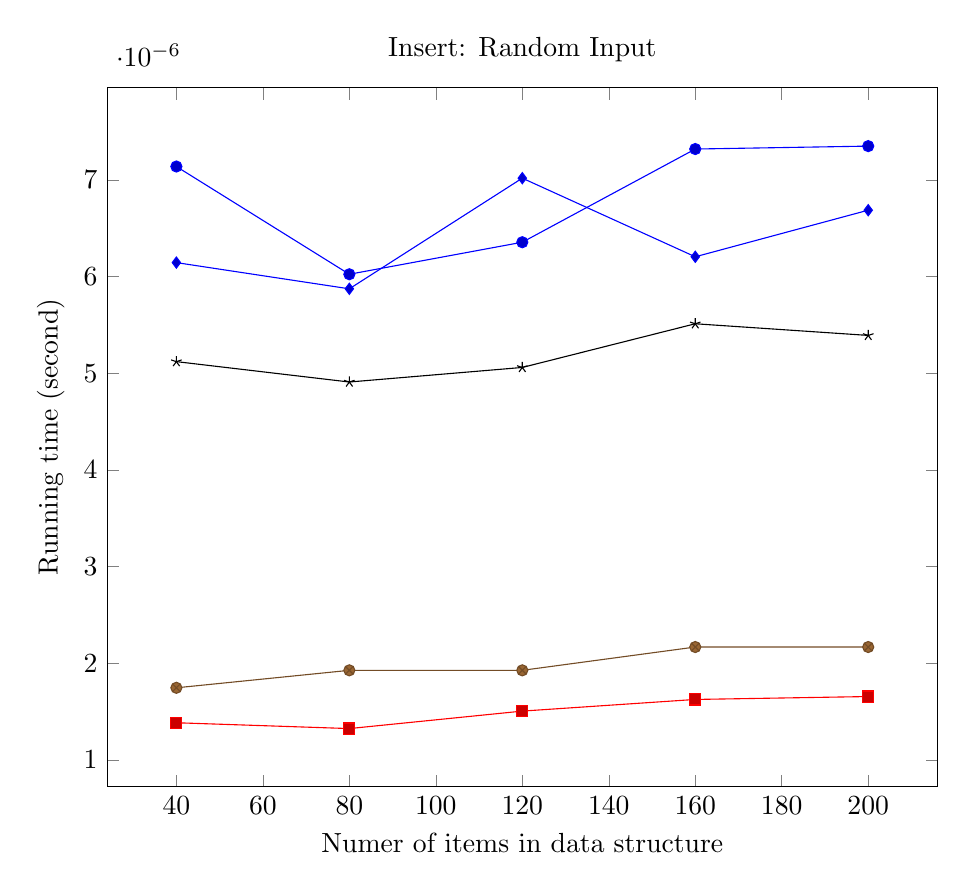
\begin{tikzpicture}
        \begin{axis}[
            xlabel={Numer of items in data structure},
            ylabel={Running time (second)},
            title={Insert: Random Input},
            width=\textwidth
        ]
		\addplot coordinates {
			(40, 7.1378554810763715e-06)
			(80, 6.023506735175488e-06)
			(120, 6.354799605290396e-06)
			(160, 7.318560682989528e-06)
			(200, 7.348678216700933e-06)
		};
		\addplot coordinates {
			(40, 1.3854065489482537e-06)
			(80, 1.3251714815254444e-06)
			(120, 1.505876683793872e-06)
			(160, 1.6263468186394902e-06)
			(200, 1.6564643523508948e-06)
		};
		\addplot coordinates {
			(40, 1.7468169531298372e-06)
			(80, 1.9275221553982645e-06)
			(120, 1.9275221550429935e-06)
			(160, 2.16846242473423e-06)
			(200, 2.16846242473423e-06)
		};
		\addplot coordinates {
			(40, 5.1199807248991645e-06)
			(80, 4.909157989274604e-06)
			(120, 5.059745657476355e-06)
			(160, 5.511508662436882e-06)
			(200, 5.391038527591263e-06)
		};
		\addplot coordinates {
			(40, 6.143976869665835e-06)
			(80, 5.872919066618465e-06)
			(120, 7.017385346230754e-06)
			(160, 6.204211937088644e-06)
			(200, 6.686092475760575e-06)
		};
        \legend{}
        \end{axis}
    \end{tikzpicture}
    \caption{Average of 0 operations, benchmarked every 0, starting at 0.}
\end{figure}